\documentclass{article} % For LaTeX2e
\usepackage{cos424,times}
\usepackage{url}
\usepackage{graphicx}
\usepackage{hyperref}
\usepackage{amssymb}

\def\Na{Na\"ive}

\title{Creating an Automated Classifier to Approximate the By-eye
  Selection of HAT Exoplanet Candidates}


\author{
Will Coulton \\
Department of Physics \\
Princeton University\\
\texttt{wcoulton@princeton.edu} \\
\And
Joshua Wallace\\
Department of Astrophysical Sciences\\
Princeton University\\
\texttt{joshuajw@princeton.edu} \\
}

\newcommand{\fix}{\marginpar{FIX}}
\newcommand{\new}{\marginpar{NEW}}

\begin{document}

\maketitle

\begin{abstract}
A proposal to use machine learning techniques to aid in the binary classification of data from the Hungarian Automated Telescope (HAT) arrays.  The HAT arrays are designed to detect periodic dimmings of stars, potentially caused by orbiting planets around those stars.  There are many signals, both physical and spurious, that can approximate planet signals, so it is important to weed out as many false positives as possible.  After an automated pipeline removes probable false planets, a final manual by-eye selection is made to create the final set of planet cadidates.  We propose to train classifier models to approximate this by-eye selection with the hope of finding a sufficiently well-performing model that can stand as a proxy for or even entirely replace the manual portion of the selection pipeline.
\end{abstract}

\section{Introduction}

The field of exoplanets (``extra-solar planets'', or planets around other stars) has established itself as the hot new field in astrophysics. Since the discovery of the first exoplanets in the early 1990's \cite{pulsarplanet}, nearly 3000 exoplanets have been discovered \cite{exoplanetorg}, with potentially thousands more exoplanets remaining unconfirmed or thus far undiscovered in existent data.  This explosion in exoplanet discovery has been fueled by the funding and construction of many exoplanet detection surveys.  The majority of exoplanets have been found by the space-based {\it Kepler} telescope and its primary \cite{kepler} and ``K2'' surveys \cite{k2}.  Ground-based surveys, while not as sensitive to smaller planets as {\it Kepler} (due to atmospheric distortion of image quality and other problems associated with observing from the ground), are sufficiently sensitive to discover Jupiter-sized planets on short-period orbits.  Such planets are called ``hot Jupiters'' because they are the similar in size to Jupiter but are sufficiently close in to the stars they orbit (much closer than Mercury is to our sun) that the star heats them up to several thousands of degrees Celsius.

  Since ground-based surveys are much cheaper to run per area of sky monitored than spaced-based surveys, the majority of known hot Jupiters have been discovered by large-scale ground-based surveys.
Of the few hundred hot Jupiters that have been found to date, the plurality (${\sim}$100) have been found by Princeton's own Hungarian-made Automated Telescope (HAT) collaboration, headed by Prof. Gaspar Bakos of the Department of Astrophysical Sciences.  This collaboration runs two surveys. The longest-running of the two surveys is HATNet, a collection of five telescopes in Arizona and two telescopes in Hawaii \cite{hatnet}.  The other survey is HATSouth, which consists of three locations with eight telescopes each: Chile, Namibia, and Australia \cite{hatsouth}.  A third survey, HATPI, which will consist of 63 telescopes in Chile, is currently being constructed \cite{hatpi}.  The telescopes themselves are small as telescopes go: only about 10 cm across, they are more similar to camera lenses than the ``normal'' telescopes usually associated with astronomy.  Figure~\ref{hsscopes} shows a picture of four of the HAT-South telescopes.

\begin{figure}
\begin{centering}
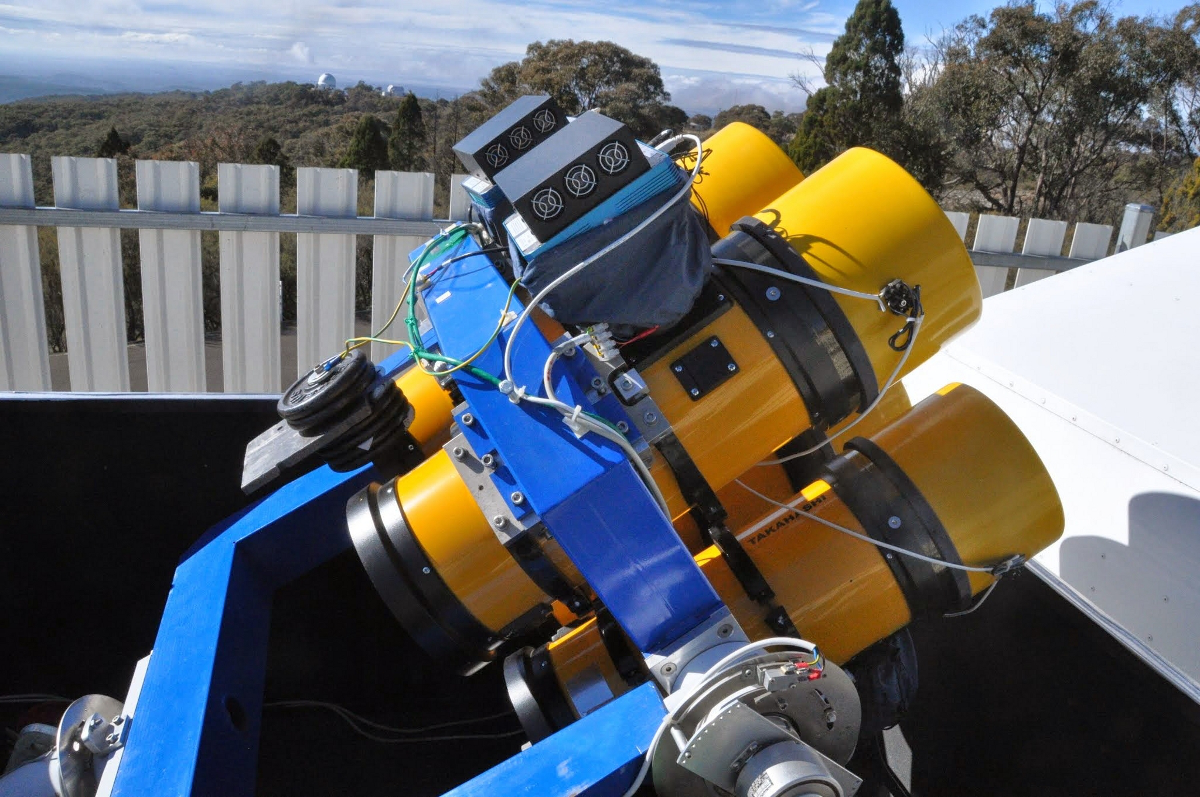
\includegraphics[width=3in]{hs-scopes.png}
\caption{\label{hsscopes} The four HATSouth telescopes at Siding Springs Observatory, Australia.  Photo credit Gaspar Bakos.  From \cite{hatsouthpicture}.}
\end{centering}
\end{figure}

The detection technique used by HAT*, {\it Kepler}, and many other exoplanet surveys is the ``transit'' technique.  Planets are far too faint compared to their host stars to be able to directly image around most stars.  Instead, in the transit technique, the brightness of stars is monitored as a function of time (usually by taking periodic long-exposure photographs of large areas of the sky).  When a planet crosses in front the star it orbits, the amount of light detected from that star is decreased.  This is demonstrated cartoon-style in Figure~\ref{transit}.  Transits are found in data using matched filtering (with either a box- or trapezoid-shaped filter, matching the signal from a transiting exoplanet), folding the data on a variety of periods and phases.  When a star is found to have periodic dips in brightness, it is labeled as a potentially planet-hosting star.  However, transiting planets are not the only source of periodic signals like that seen in Figure~\ref{transit}.  Starspots rotating in and out of view also provide periodic dips in brightness and binary stars that eclipse each other in a grazing way (so the amount of light that goes missing during an eclipse is about the same as a planet) are two examples of astrophysical false positive signals. Various cuts are made to help ensure that a prospective planet is neither any of these false positives nor a spurious signal.  The various parameters of the fit to the transit signal (depth, time of ingress, length of transit) are often good indicators to separate between planet and not.  These cuts are automated.  However, after the cuts, there are still false positives that are not apparent to the pipeline but are obvious to a trained human eye.  Thus, the final step in the HAT pipeline is a manual, by-eye examination of the signal.  Planet candidates that pass this step then are sent for follow up (and hopefully confirmation!) at bigger telescopes.

\begin{figure}
\begin{centering}
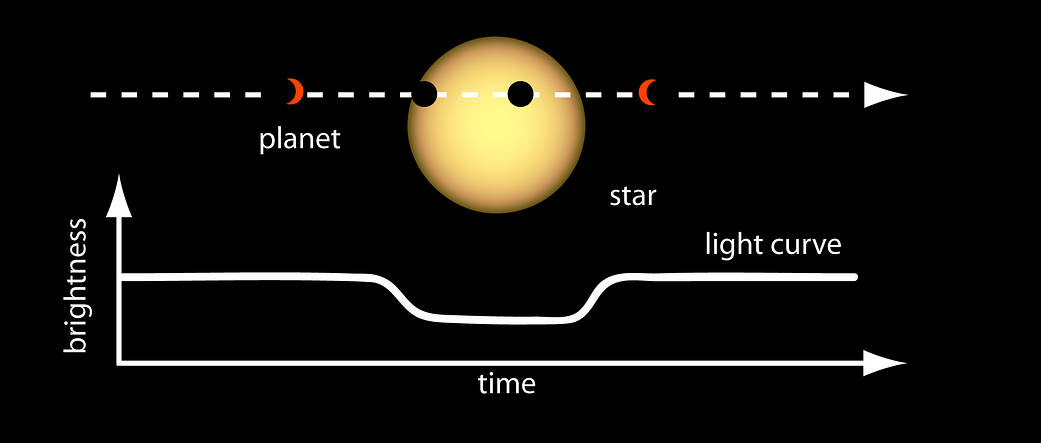
\includegraphics[height=1.9in]{transit.png}
\caption{\label{transit} An example ``light curve'' (brightness as a function of time) from a star that hosts a transiting exoplanet.  As the planet crosses in front of the star, the measured brightness from the star is less than the out-of-transit value.  Partial eclipses as the planet is transitioning from being out-of-transit to fully in transit put a slope in the light curve between in-transit and out-of-transit magnitudes.  Public domain image from \cite{transit_pic}.}
\end{centering}
\end{figure}

Other than this manual step, the vetting of possible planet candidates is completely automatic.  This single manual step is quite labor intensive, and prevents a fully automatic characterization of planet detection efficiency (what fraction of real planets get correctly identified), which is necessary for the calculation of statistics related to the occurrence rate of these planets.  Thus, it would be very nice to have an automated approximation to the by-eye work that has occurred.  This is the purpose of this project.


\section{Related Work}
The premier (and only statistically robust) calculation of a hot Jupiter occurrence rate from transit data is that from the primary {\it Kepler} mission \cite{howard2012}.  Because of the exquisite quality of the data from the {\it Kepler} telescope, their detection efficiency for hot Jupiters is near 100\% and they are better able to automatically identify false positives than the HAT collaboration is from our surveys.  Because of this, the {\it Kepler} pipeline needs much less manual vetting of planet candidates and thus the {\it Kepler} team has not needed to worry about the manual step as teh HAT collaboration does.  However, as mentioned before, the HAT collaboration has found more hot Jupiters than any other collaboration, and so if we can get a good handle on our detection efficiency we have the potential to provide the most precise measure of the occurrence rate of these planets, which will help inform planet formation theory.

Unfortunately, since the {\it Kepler} work did not need to worry so much about detection efficiencies and pipeline misclassifications, they did not develop the hard statistical/machine learning tools that would be useful for this work.  However, a recent astrophysics study \cite{ogle2017} that used a very similar time-series data set as the HAT surveys used a random forest classifier to classify 450,000 eclipsing binaries (binary stars that transit each other, similar to how a planet transits a star) from their data.

\section{Data}
The data used are unpublished and (currently) proprietary.  They were extracted from the HAT database using a script provided by Joel Hartman\footnote{jhartman@astro.princeton.edu}, Research Scienctist at Princeton University.  The database itself currently has no reference.

The data consists of 1024 positive cases and 29,421 negative cases of potential planet candidates that passed the manual vetting process.  The number of positive cases is perhaps too low to train a truly robust model, but it is unfortunately all we have to work with.  The process of discovering new planets is one of constant attrition, and there are unfortunately more cases of false positive signals than of real signals.  There are 92 features that consist of such measured quantities as the fit parameters to the transit dip (transit depth, length, etc.), quantities related to the power spectrum from the matched filtering, measured quantities for the star (brightness in various colors), and signal to noise measures.  All of these quantities are  continuous, not categorical.  There are some missing values: 284 ``inf'' (0.01\% of all values) and 4461 ``nan'' (0.2\% of all values).  The ``inf'' values are mostly concentrated in a single column (feature) of the data, while the ``nan'' values tend to cluster in the same rows (objects).  These data were imputed using [fill in by Will].

\section{Methods}
\section{Methods}

Our first approach to this problem will be to investigate the simple binary classifiers that we have covered in class so far. These include Naive Baye's, random forests, support vector machine (SVM), and logistic regression. With logistic regression will investigate two types of regularization using $l1$ and $l2$ penalties. We will also explore a set of feature selection methods such as mutual information.

Whilst our main goal is to predict which objects would be manually selected we are also interested in running a set of unsupervised learning algorithms to view any hidden structure in the data set. These methods will include Kmeans and gaussian mixture models. This will be useful for potentially identifying new approaches to automating this process as well as potentially probing some new relationships.

\section{Results}
\subsection{Unsupervised Learning}
There were no unsupervised methods that provided obvious structure  that matched the classifications.  For the K-means method, a variety of k-values were used.  In each case, the positive cases were divided among the categories in rough proportion to the total number of cases in each category.  A similar thing happened with LDA.  Since LDA is a mixed membership model, we decided to assign hard membership if an object had larger than a certain threshold (e.g., 0.8 or 0.9) membership in a particular topic.  Members of a particular topic were distributed between positive and negative examples in rough proportion to the actual distributions of the examples in the data set.
For PCA, the first principal component explains 20\% of the variance, then 11\%, 8.5\%, and 7.8\% for the next three principal components.  Figure~\ref{pca} shows the projection of the data onto the first two principal components.  The green circles are the positive cases and blue dots are the negative cases.  From just the first two principal components, there is no exploitable separation between the positive and negative cases that allows for classification.  Running K-means (with several different values of k) on the PCA decomposed values also revelead no exploitable structure for classification.
\begin{figure}
\begin{centering}
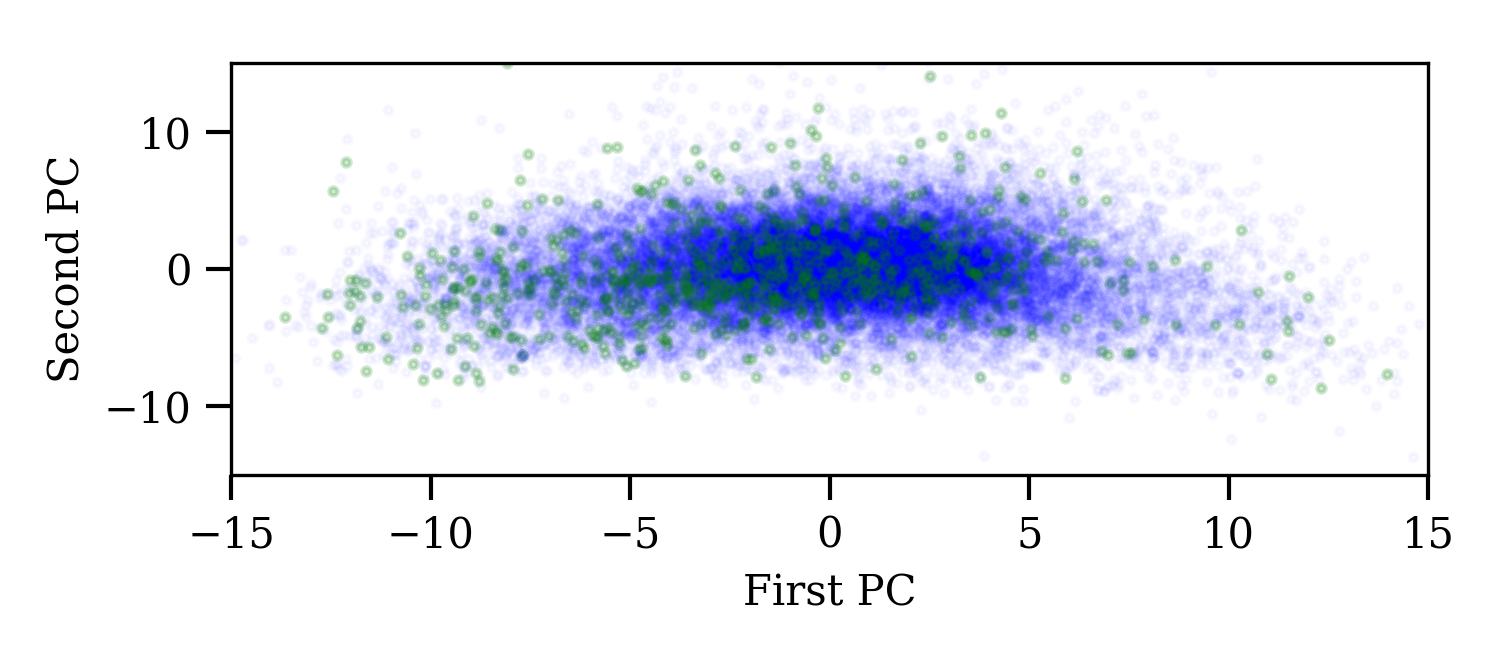
\includegraphics[width=5in]{pca.png}
\caption{\label{pca} The data projected on the first two principal components.  The positive cases are in green and the negative cases are in blue.  Note that the scales of the axes are the same; they have been stretched and squished to better fit in the single-column format of this paper.  The transparency of the green points is less than the blue points so that they could be better visible, since there are about 30 times more blue points than green points.  There is no obvious separation between the two groups of points, though the green points do have larger variance than the blue points along the first principal component (22.6 versus 17.7).  In the axis labels, ``PC'' = principal component.}
\end{centering}
\end{figure}







\subsection{Supervised Learning}


\section{Discussion and Conclusion}
In this work, I compared the performance of five different classifiers in classifying sentiment and then used six different feature selectors on the best-performing classifiers.  The best classifier was a RF classifier, while among the NB classifiers the Bernoulli estimator worked the best.  Feature selection offered only marginal improvement upon the base results.  For the NB Bernoulli classifier, a KB algorithm with an F-test scoring function performed the best, while for the RF classifier the best feature selector is a toss between KB with a $\chi^2$ scoring function and a ``by hand'' culling of the feature set that I performed.  Two of the feature selectors (KB with a mutual information scoring function and RFE) took too long to run with the RF classifier (which already took a long time to run relative to the other classifiers) to be shown in this work.

A primary future direction for this work is to increase the size of the training data.  The fact that feature selection did not do much seems to indicated that the training data have not yet saturated the useful feature set.  Another useful future direction is to expand the features from the training data already available, e.g., incorporate bigrams and not just unigrams.  A final suggestion is to study possible synergies between the different classifiers; perhaps using multiple of them together would reveal a whole that is greater than the sum of its parts.

\subsubsection*{Acknowledgments}
We are grateful to Joel Hartman for providing a script to extract the
necessary data from the HAT database.  We are also grateful to the
entire HAT team (PI: Gaspar Bakos) for their many dedicated years of
constant observations and the huge pile of astronomical data they've collected.


\bibliography{ref}
\bibliographystyle{plain}

\end{document}
